%\documentclass[11pt]{article}
\documentclass[print,phd_com]{nuthesis}
%\usepackage{times}

%\setlength{\textwidth}{6.5in}
%\setlength{\textheight}{9.0in}
%\setlength{\topmargin}{-.5in}
%\setlength{\oddsidemargin}{-.0600in}
%\setlength{\evensidemargin}{.0625in}

\newcommand{\secref}[1]{Section~\ref{#1}}
\usepackage{xcolor}
\usepackage{setspace}
%\usepackage{algorithmic}
\usepackage{amsmath}
\usepackage{amssymb}
\usepackage{cite}
\usepackage{textcomp}
\usepackage{float}
\usepackage{caption}
%\usepackage{algorithm}
\usepackage{url}
%SPAWC-2018
\usepackage{color}
\usepackage{enumitem}

\usepackage[pdftex]{graphicx}
\usepackage{graphicx,subfig}
\usepackage{calc}
\usepackage{url}
\usepackage{listings}
\usepackage{subfig}
\usepackage{multirow}
\usepackage{bbding}
\usepackage{rotating}
\usepackage{array}
\usepackage{float}

%SPAWC-2018
\usepackage{graphics}
\usepackage{mathtools}
\usepackage{bigints}
\usepackage{float}
\usepackage{caption}
%\usepackage{subcaption}
\usepackage[ruled, linesnumbered]{algorithm2e}
%\usepackage[linesnumbered,lined,boxed,commentsnumbered]{algorithm2e}
\usepackage{algpseudocode}
\usepackage[pdftex]{graphicx}
\usepackage{epstopdf}
\graphicspath{{./figures/}}
\usepackage[version=4]{mhchem}

\newlength{\imgwidth}

\newcommand\scalegraphics[1]{%   
    \settowidth{\imgwidth}{\includegraphics{#1}}%
    \setlength{\imgwidth}{\minof{\imgwidth}{\textwidth}}%
    \includegraphics[width=\imgwidth]{#1}%
}


\begin{document}
\frontmatter
\title{Molecular Communication in Biological Cells: Foundational Study and Development of Computational Techniques }
\author{Zahmeeth Sayed Sakkaff}
\adviser{Massimiliano Pierobon, Chair \\ Myra B. Cohen \\ Juan Cui \\ Tomas Helikar \\ Christopher Henry}

\adviserAbstract{Massimiliano Pierobon}
\major{Computer Engineering}
\degreemonth{May 15}
\degreeyear{2018}


\maketitle
%IF NEEDED ACTIVAT TO HAVE AN ABSTRACT
%\begin{center}
%\huge\bfseries{Abstract}
%\end{center}
%
%
%\begin{abstract}
%
%
%\end{abstract}


\begin{acknowledgments}
Your ack
\end{acknowledgments}


%\newpage
\tableofcontents
\newpage
\listoffigures
\listoftables

% \doublespace
\mainmatter
\chapter{Introduction}
\label{sec:Introduction}
\par Your Inro

\chapter{Background}
\section{Motivation}
\label{sec:motivation}
\par Your Motivation

\section{Biological Pathways}
\label{sec:biologicalpathways}
\par Your Details
\begin{figure} [H]%[!th]
	\begin{center}
		\centering
		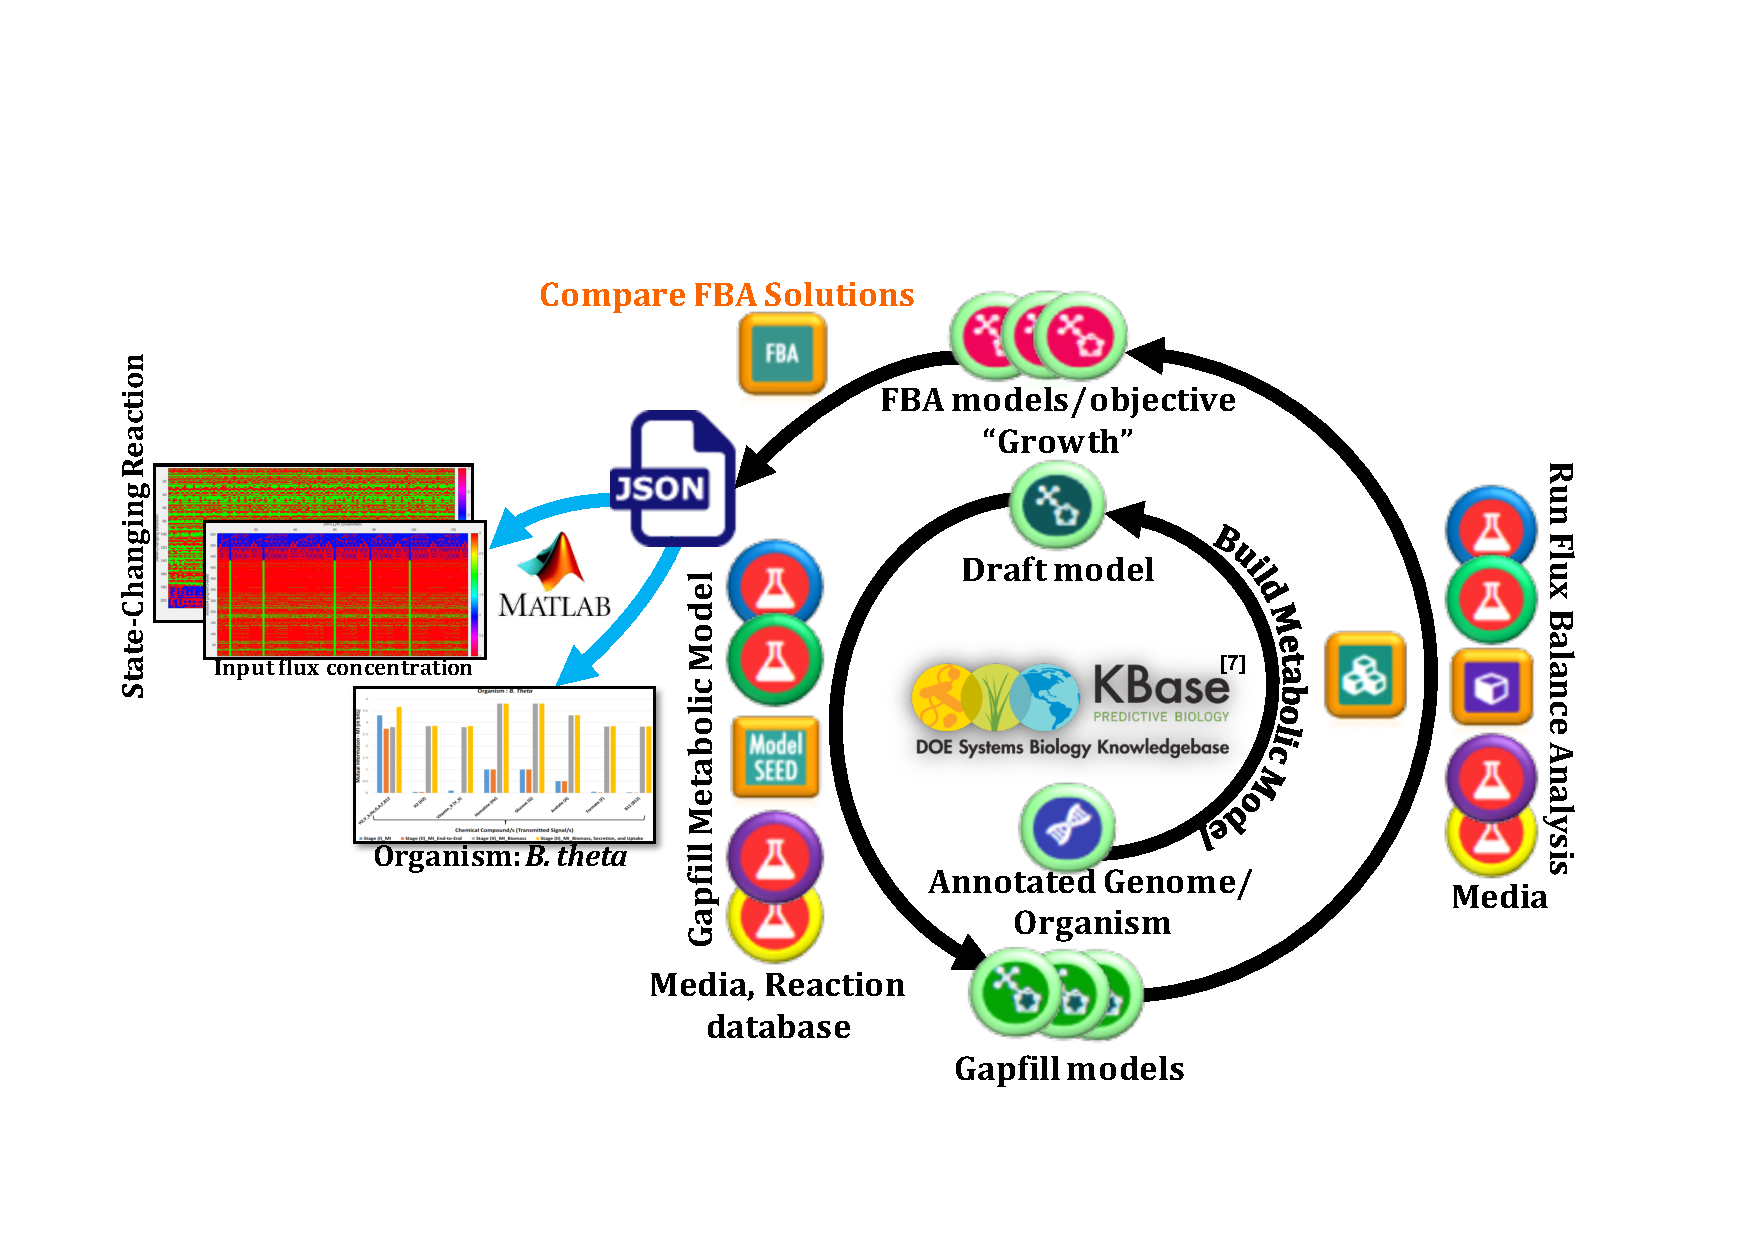
\includegraphics[width=\linewidth]{ZSworkflow.pdf}
		\caption{Graphical representation of the interconnection of signal transduction, gene regulation and metabolic pathways.}
		\label{fig:biologicalpathways}
		\vspace{-0.3in}
	\end{center}
\end{figure}

\subsection{Signal Transduction}
\label{subsec:signaltransdution}
\par Your subsection

ll's internal biological pathways. The main challenges in achieving this goal is a follows:
\begin{itemize}
\item AAA
\item BBB
\end{itemize}
\chapter{Molecular Communication in Cell Metabolism}
\label{sec:MCinCellMetabolism}
\par Reference~\cite{gonccalves2013bridging}.

%equation
\begin{eqnarray} \label{eqn:enzyme_regulation_logic}
r_i &\simeq& \beta H \left( [TF^{*}] - K_d \right) \; \mathrm{if~activation} \, , \\
r_i &\simeq& \beta H \left( K_d - [TF^{*}] \right) \; \mathrm{if~repression} \, ; \nonumber
\end{eqnarray}
equation reference~\eqref{eqn:enzyme_regulation_logic}.


\chapter{Conclusion}
\label{sec:Conclusion}
\backmatter


\section{Proposed Timeline}
The future research is planned in a 16-20-month timespan, and consists of the following five phases as shown in Table~\ref{table:Timeline}. This plan may be subject to changes based on the circumstances. 
\begin{table} [H]
	\centering
	\caption{Proposed Timeline.}
	\vspace{-0.1in}
	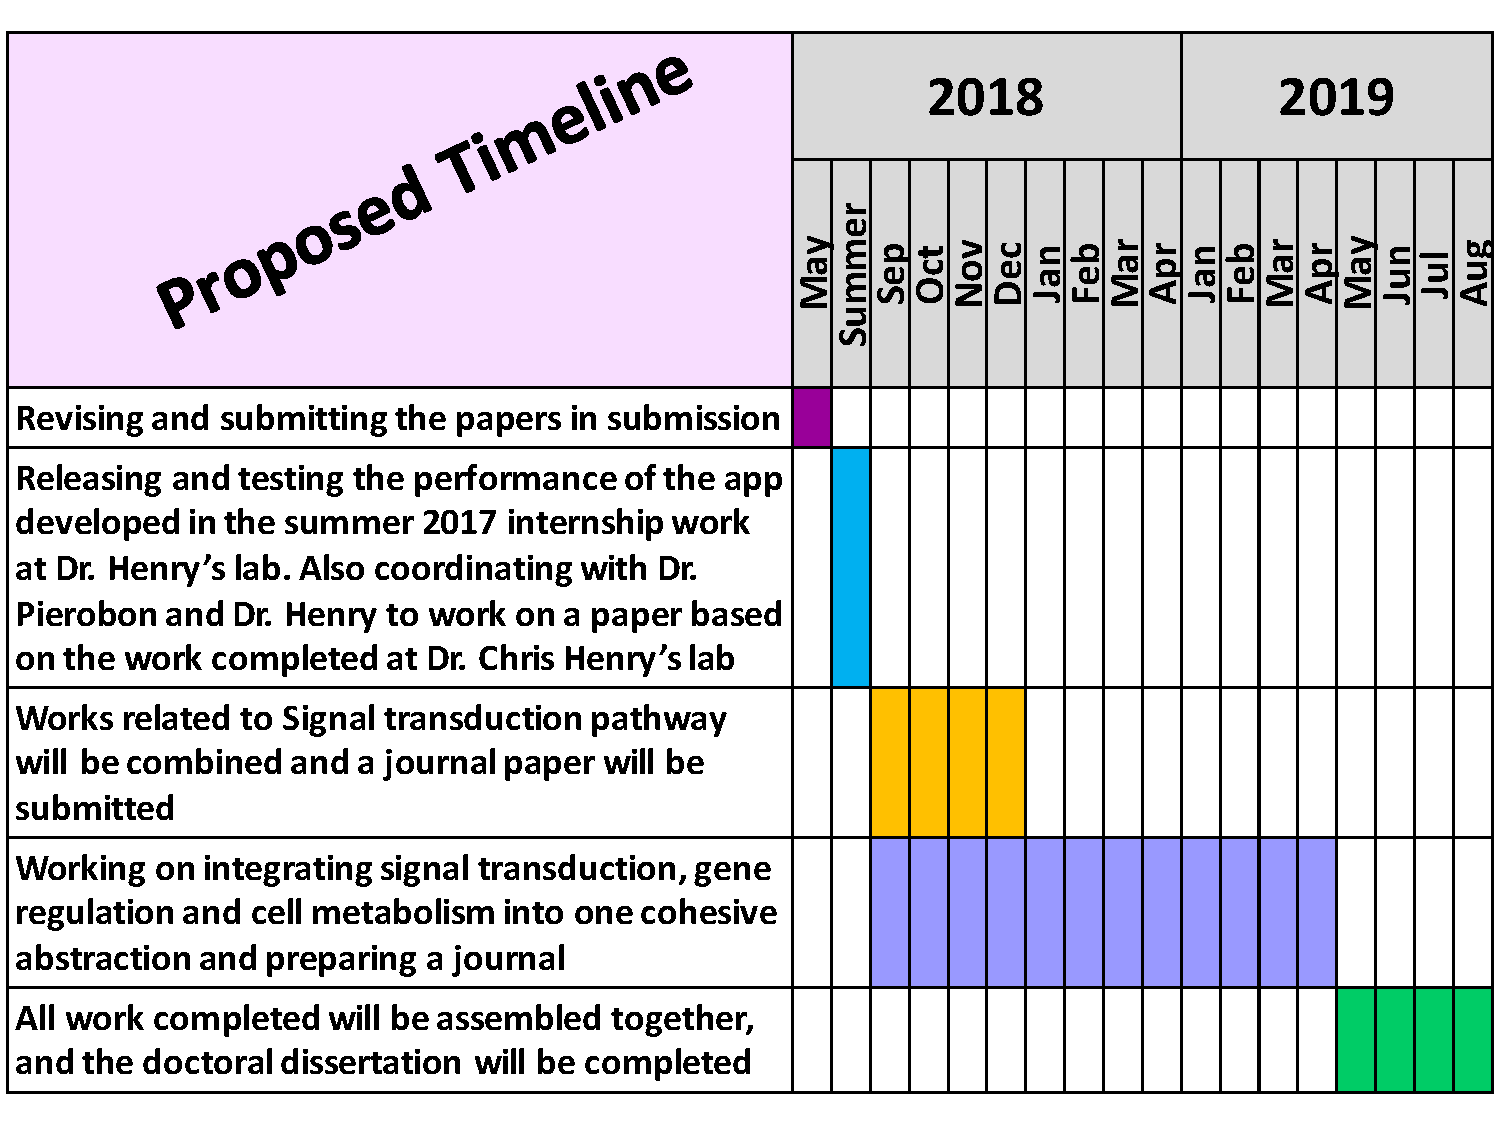
\includegraphics[width=\linewidth]{Comprehensive_Timeline.pdf}
	\label{table:Timeline}
\end{table}

\bibliographystyle{plain}
\bibliography{nano,ZSDissertation,nano_2, nano_ZS}

\end{document}

\endinput

